%       \documentclass[11pt]{beamer}
\documentclass[11pt]{beamer}
%aspectratio=1610
%default font size 11pt;8pt, 9pt, 10pt, 11pt, 12pt, 14pt, 17pt, 20pt
%\usetheme[compress]{Singapore} %title at the top
%\usecolortheme{freewilly}
\usetheme[compress]{Madrid}
%\usetheme[compress]{CEA}
%transparency
% \beamertemplatetransparentcoveredhigh
%\beamertemplatetransparentcovereddynamicmedium

\usepackage[T1]{fontenc}
%       \mode<article> % 仅应用于article版本
%       {
%       \usepackage{beamerbasearticle}
%       \usepackage{fullpage}
%       \usepackage{hyperref}
%       }

%font theme
%\usefonttheme[onlymath]{serif}
% \usefonttheme{structureitalicserif}
% \usefonttheme{structurebold}
% \usefonttheme{structuresmallcapsserif}
% \usepackage{lucidaso} % Lucida Bright (SO Version)
\usefonttheme[onlymath]{serif}
%\usepackage[small]{eulervm} % Euler VM for math font
%\usepackage{helvet}


%color themes:albatross crane beetle dove fly seagull wolverine beaver
% \usecolortheme{fly}
%Outer color themes:whale, seahorse, dolphin
\usecolortheme{whale}
% Inner color themes: lily, orchid,rose
\usecolortheme{orchid}

%rectangles circles inmargin rounded
\useinnertheme{rectangles}
%\useinnertheme[shadow]{rounded} % 对 box 的设置: 圆角、有阴影.
%infolines miniframes shadow sidebar c smoothtree split tree progressbar
\useoutertheme{progressbar}

%define colors
\setbeamercolor{uppercol}{fg=white,bg=blue}%
%\setbeamercolor{lowercol}{fg=black,bg=gray}%
\xdefinecolor{lavendar}{rgb}{0.8,0.6,1}
\xdefinecolor{olive}{cmyk}{0.64,0,0.95,0.4}
\colorlet{structure}{green!60!black}
%redefine structure color
%\usecolortheme[named=yellow]{structure}
%redefine alert color
%\setbeamercolor{alerted text}{fg=cyan}


\setbeamertemplate{headline}[default]
%\setbeamertemplate{navigation symbols}{}
\mode<beamer>{\setbeamertemplate{blocks}[rounded][shadow=true]}
\setbeamercovered{transparent}
\setbeamercolor{block body example}{fg=blue, bg=black!20}

\beamertemplateballitem

%\beamertemplateshadingbackground{blue!5}{yellow!10}

\usepackage{pifont}
%\usepackage{textcomp}

%\usepackage{pgf,pgfarrows,pgfnodes,pgfautomata,pgfheaps}
\usepackage{amsmath}
\usepackage{amsfonts}
\usepackage{amssymb}
\usepackage{boxedminipage}


\usepackage{graphicx}

%shadowbox,fbox,Ovalbox,ovalbox,doublebox
\usepackage{fancybox}
\usepackage{multimedia}
\usepackage{listings}
\usepackage{boxedminipage}
% \usepackage{babel}
%\usepackage{enumitem}


\title[eXpress]{Diagnosing Performance Changes by Comparing Request Flows}
\author{Raja Sambasivan, et al.}
\institute{Presented by\\ Mingrui Zhang(1110379057)\\ Hongxu Chen(1110379002)}
\date[\today]{\today}
\subject{}

% \AtBeginSection[]{ % 在每个Section前都会加入的Frame
% \frame<handout:0>{
% \frametitle{Outline}
% \tableofcontents[current,currentsubsection]
% }
% }
% \AtBeginSection[]{%
%   \begin{frame}<beamer>
%     \frametitle{Outline}
%     \tableofcontents[sectionstyle=show,subsectionstyle=hide]
%   \end{frame}
%   \addtocounter{framenumber}{-1}% If you don't want them to affect the slide number
% }

\RequirePackage{ifthen}
\newboolean{sectiontoc}
\setboolean{sectiontoc}{true} % default to true

\AtBeginSection[]
{
\ifthenelse{\boolean{sectiontoc}}{
\begin{frame}<beamer>{Outline}
\tableofcontents[currentsection]
\end{frame}
\addtocounter{framenumber}{-1}
}
}

%\setbeamertemplate{navigation symbols}{}

\hypersetup{pdfpagemode={FullScreen}}
%\hypersetup{pdfstartview={FitH}}

\begin{document}


%\frame[plain]{\titlepage} % 产生主题页,plain选项表示不显示页眉页脚等内容
\frame{\titlepage}

\part{Introduction}
\frame{\partpage}
\section{Difficulties}
\begin{frame}
\frametitle{\secname}
\shadowbox{Performance problems in distributed systems}
\begin{itemize}
  \item May have many root causes
  \item May be contained in any one or more of the component processes
  \item May emerge from the interactions among component processes
\end{itemize}
\end{frame}


\begin{frame}
\frametitle{An Example}
\only<1>{\shadowbox{Example}\\
\begin{itemize}
  \item[] {Debugging a feature addition}
  \item[]
  \begin{center}
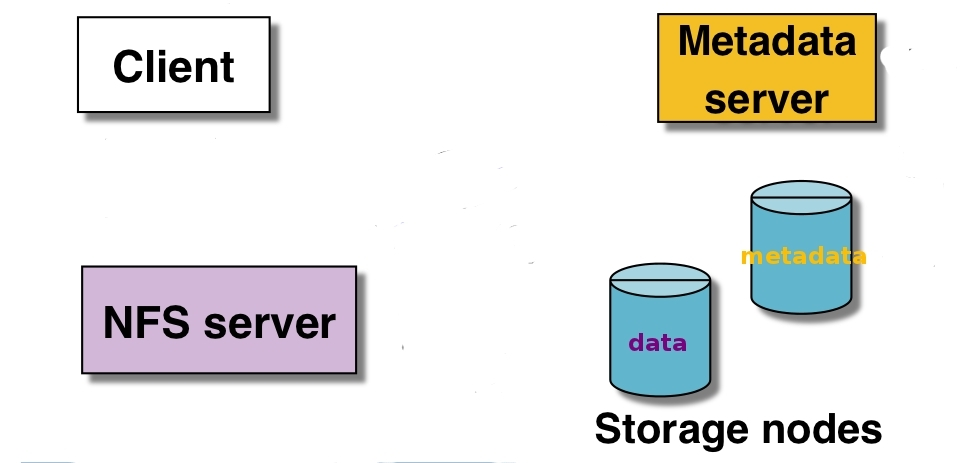
\includegraphics[height=5cm]{fig/artchitecture_original.jpg}
\end{center}
\end{itemize}
}
\only<2>{\shadowbox{Before addition}\\
\begin{itemize}
  \item[] Every file access needs a MDS access
  \item[]
  \begin{center}
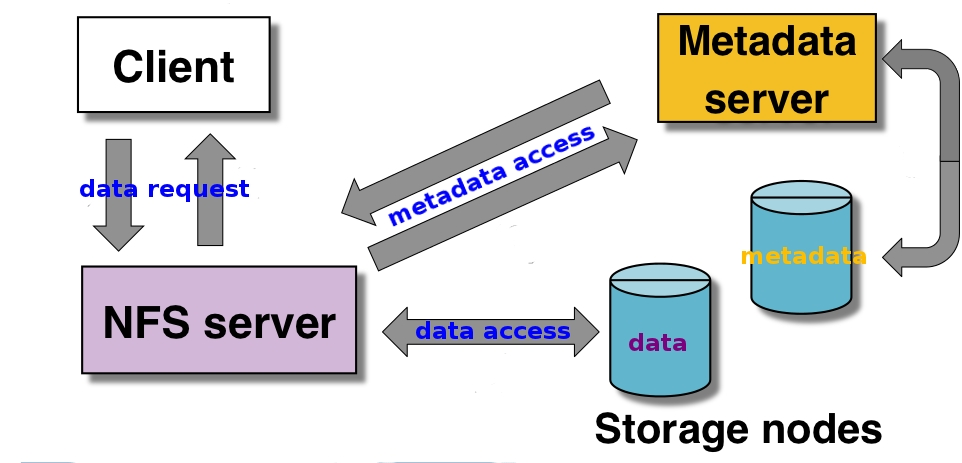
\includegraphics[height=5cm]{fig/artchitecture.jpg}
\end{center}
\end{itemize}
}
\only<3>{\shadowbox{After: Metadata prefetched to clients}\\
\begin{itemize}
  \item[] Most requests \emph{don't} need MDS access
  \item[]
  \begin{center}
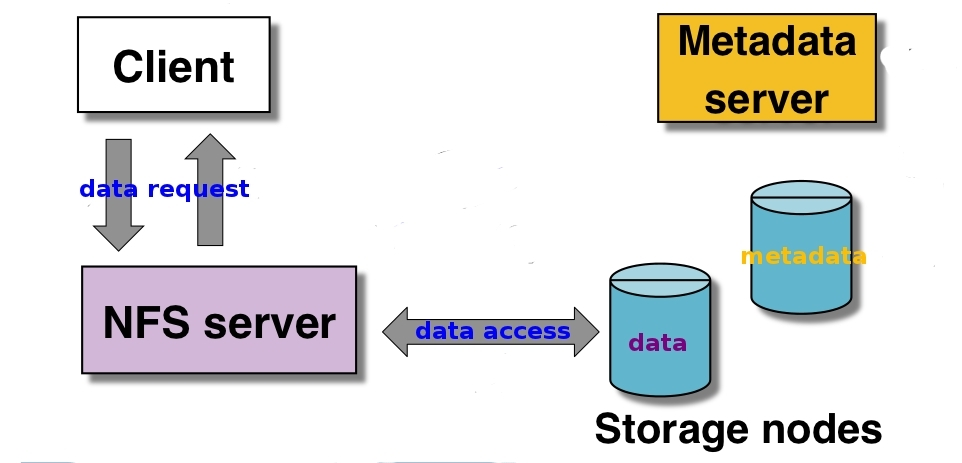
\includegraphics[height=5cm]{fig/artchitecture_final.jpg}
\end{center}
\end{itemize}
}
\end{frame}

\begin{frame}
\frametitle{Debugging a feature addition}
\begin{itemize}
  \item<1>Adding metadata prefetching reduced performance instead of improving
  it
  \vskip18pt
  \item<2>How to efficiently diagnose this?
\end{itemize}
\end{frame}

\section{Request Flow Comparison}

\begin{frame}
\frametitle{Request-flow comparison will show}
\hypertarget{prefetching}
\beamergotobutton{\hyperlink{evaluation}{Jump to evaluation}}
\only<1>{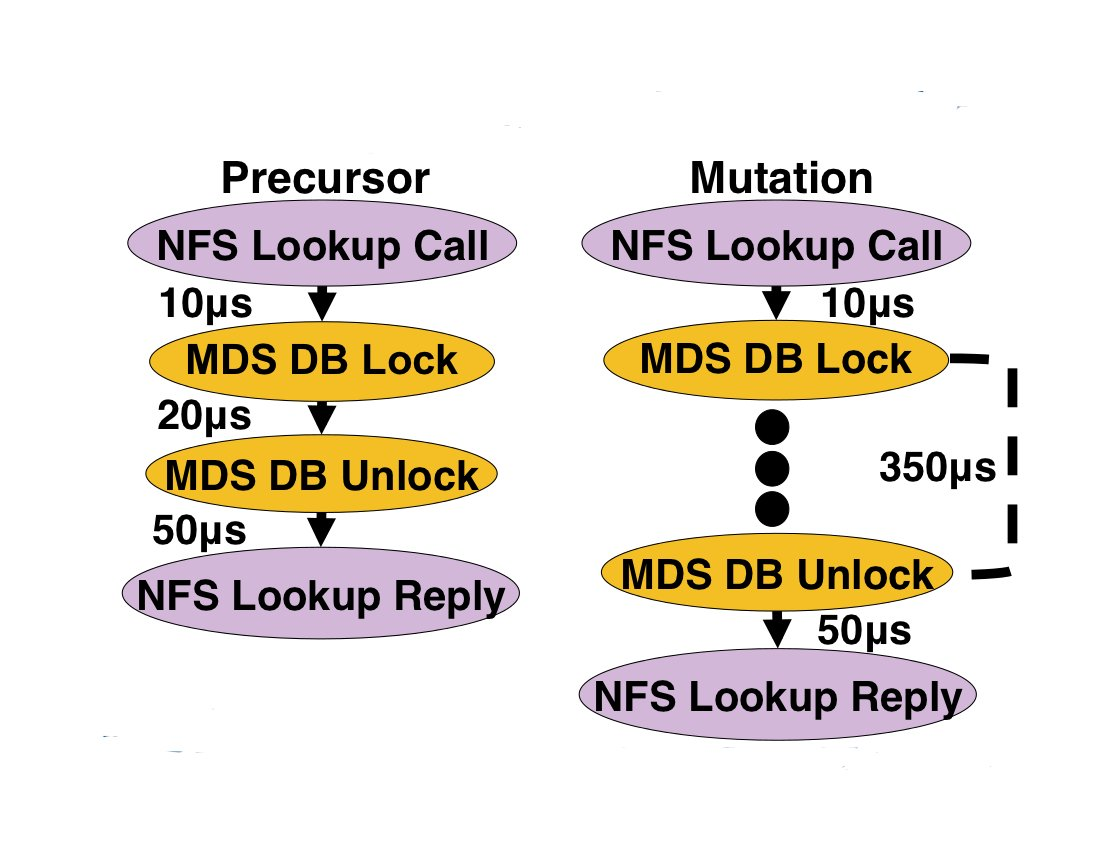
\includegraphics[width=0.9\textwidth]{fig/show1.jpg}}
\only<2>{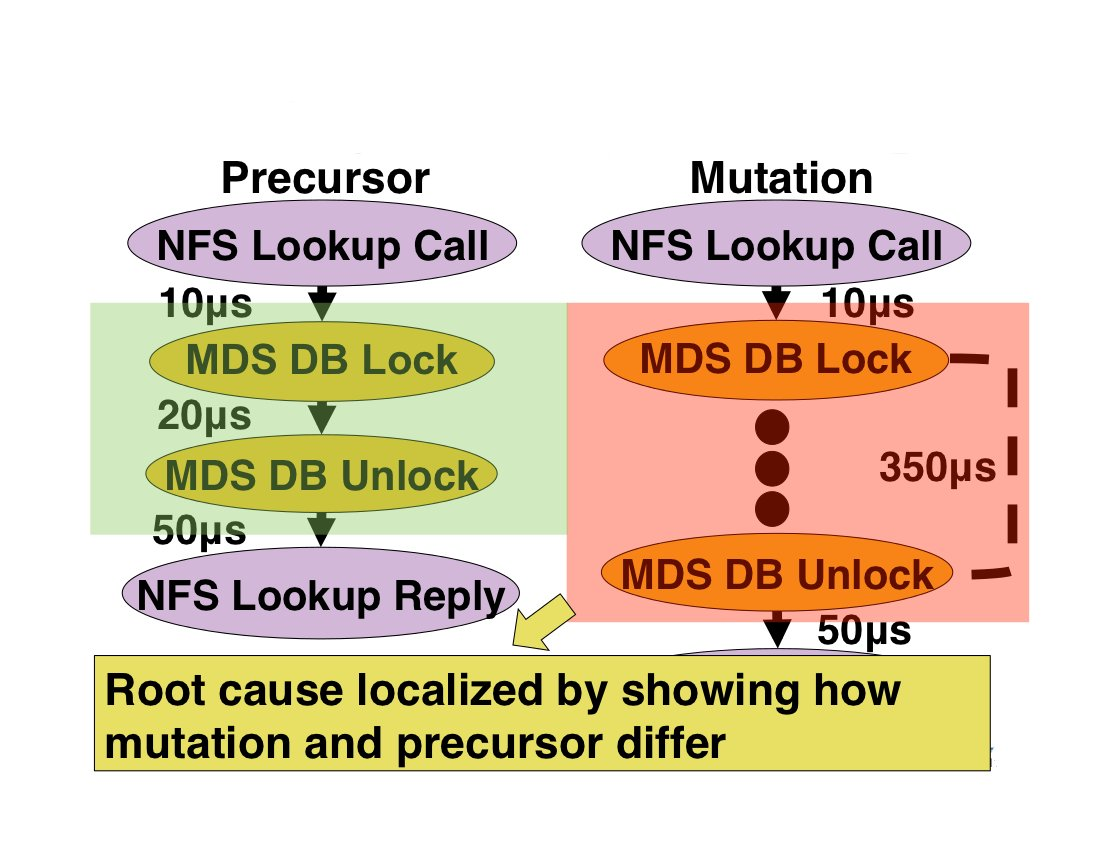
\includegraphics[width=0.9\textwidth]{fig/show2.jpg}}
\end{frame}

\begin{frame}
\frametitle{Request Flow Comparison}
\begin{itemize}
  \item<1-> Identifies distribution changes
  \begin{enumerate}
    \item[\ding{43}] Distinct from anomaly detection
    \item[--] E.g. Magpie, Pinpoint, etc.
  \end{enumerate}
  \vskip11pt
  \item<2> Satisfies many use cases
  \begin{enumerate}
    \item[\ding{43}]Performance regressions/degradations
    \item[\ding{43}]Eliminating the system as the culprit
  \end{enumerate}
\end{itemize}
\end{frame}

\begin{frame}
\frametitle{Contributions}
\begin{itemize}
  \item<1-> Heuristics for identifying mutations,precursors, and for ranking them
  \begin{enumerate}
    \item[\ding{45}] Implementation in Spectroscope
  \end{enumerate}
  \vskip11pt
  \item<2> Use of Spectroscope to diagnose
  \begin{enumerate}
    \item[\ding{44}]Unsolved problems in Ursa Minor
    \item[\ding{44}]Problems in Google services
  \end{enumerate}
\end{itemize}
\end{frame}

\part{Spectroscope Workflow}
\frame{\partpage}

\section{Overview}
\begin{frame}
\frametitle{\secname}
\begin{columns}
\column{.5\textwidth}
\begin{itemize}
  \item Input: two periods of activity
  \begin{enumerate}
    \item non-problem period graph
    \item a problem period graph
  \end{enumerate}
  \item Categrazation
  \begin{enumerate}
    \item Response time mutation
    \item Structural mutation and precursor
  \end{enumerate}
  \item Ranking by expected contribution to the performance change
  \item Visulation
\end{itemize}
\column{.48\textwidth}
\begin{figure}[htbp]
\centering
% 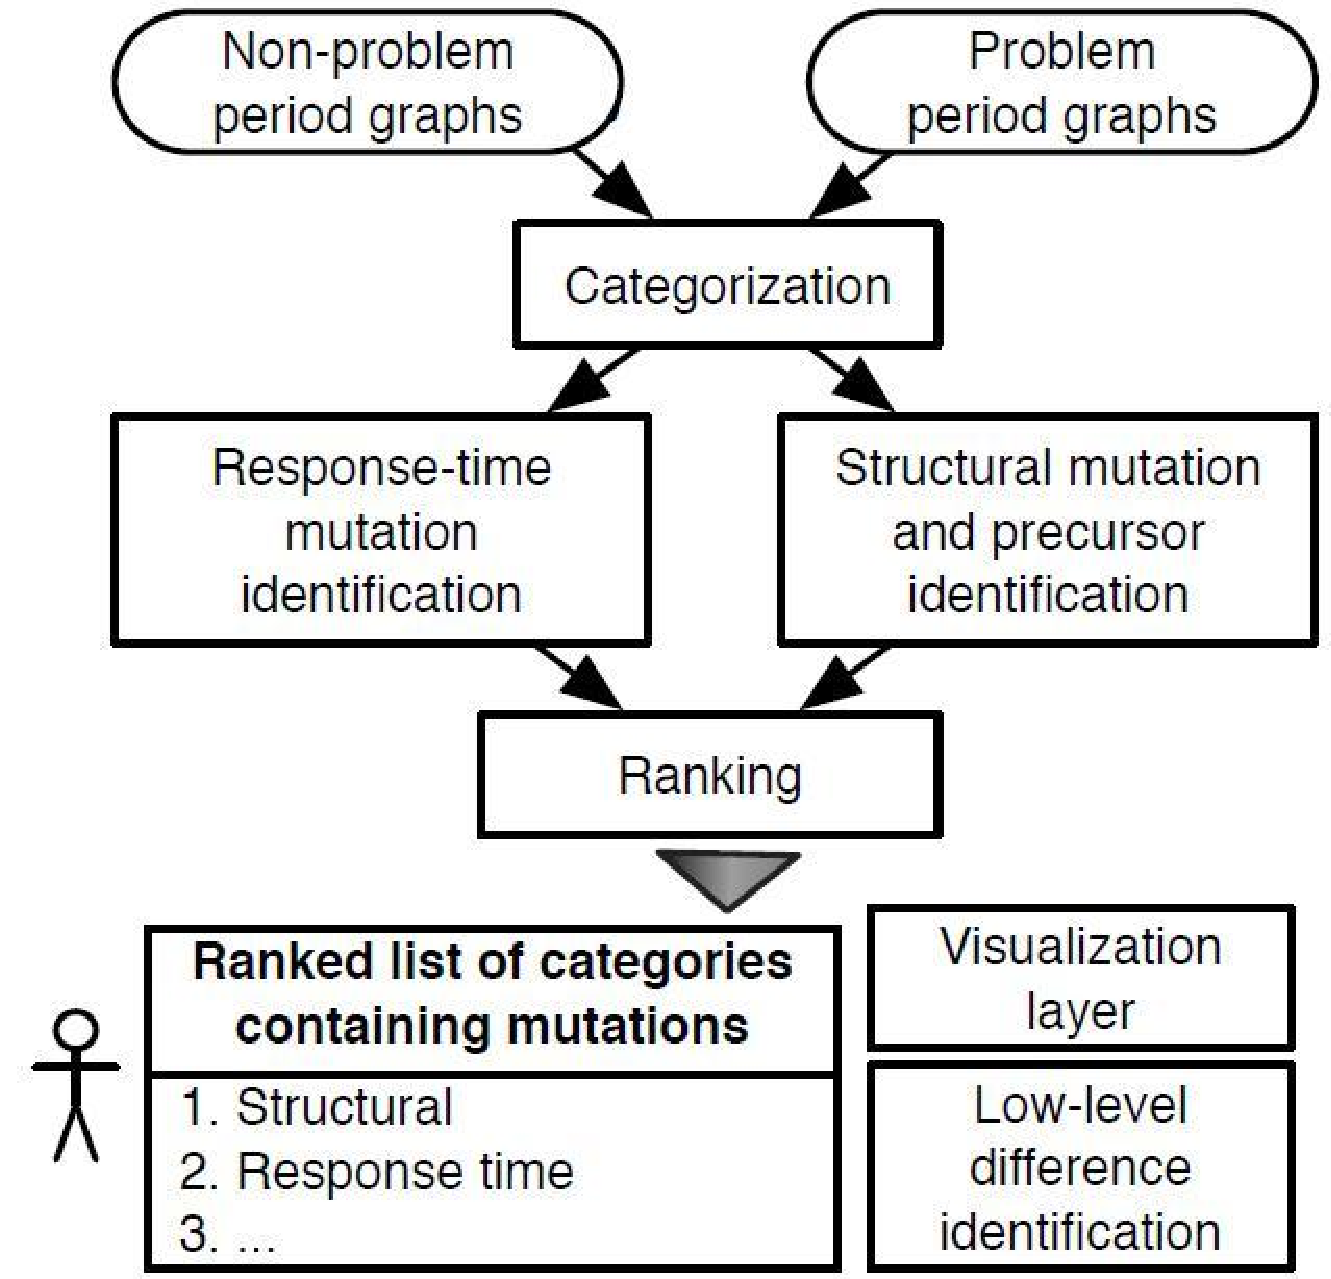
\includegraphics[width=\textwidth]{fig/workflow.pdf}
\caption{Spectroscope's workflow for comparing request flows}
\label{fig:workflow}
\end{figure}
\end{columns}
\end{frame}

\section{Input}

\begin{frame}
\frametitle{Spectroscope workflow (\romannumeral 1)}
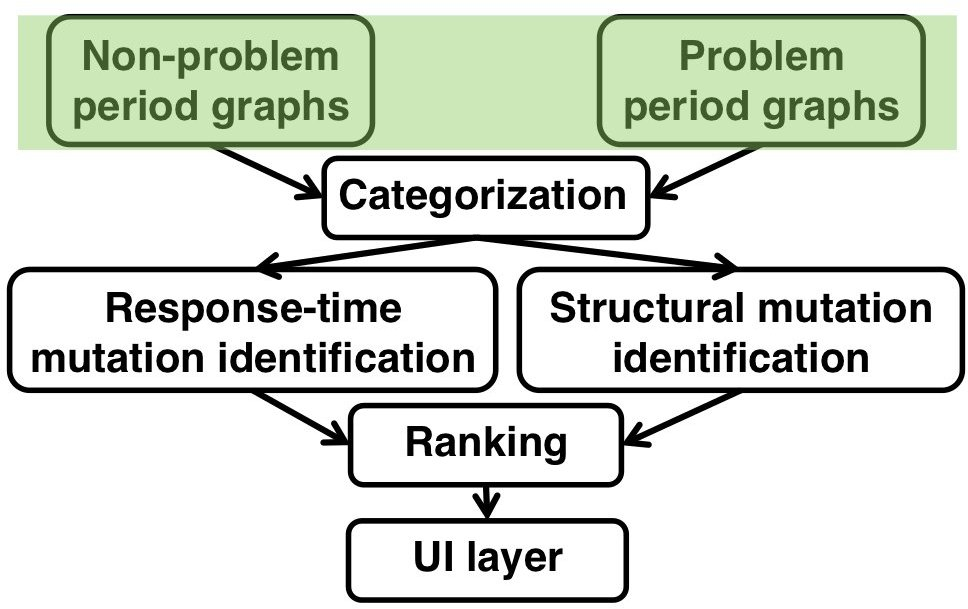
\includegraphics[width=\textwidth]{fig/work1.jpg}
\end{frame}

\begin{frame}
\frametitle{Graphs via end-to-end tracing}
\begin{itemize}
  \item Used in research \& production systems
  \item Works as follows:
  \begin{enumerate}
    \item Tracks trace points touched by requests
    \item Request-flow graphs obtained by stitching together trace points accessed
  \end{enumerate}
  \item Yields $<1\%$ overhead request sampling
\end{itemize}
\end{frame}

\begin{frame}
\frametitle{Example: Graph for a striped read}
\begin{columns}
\column{.7\textwidth}
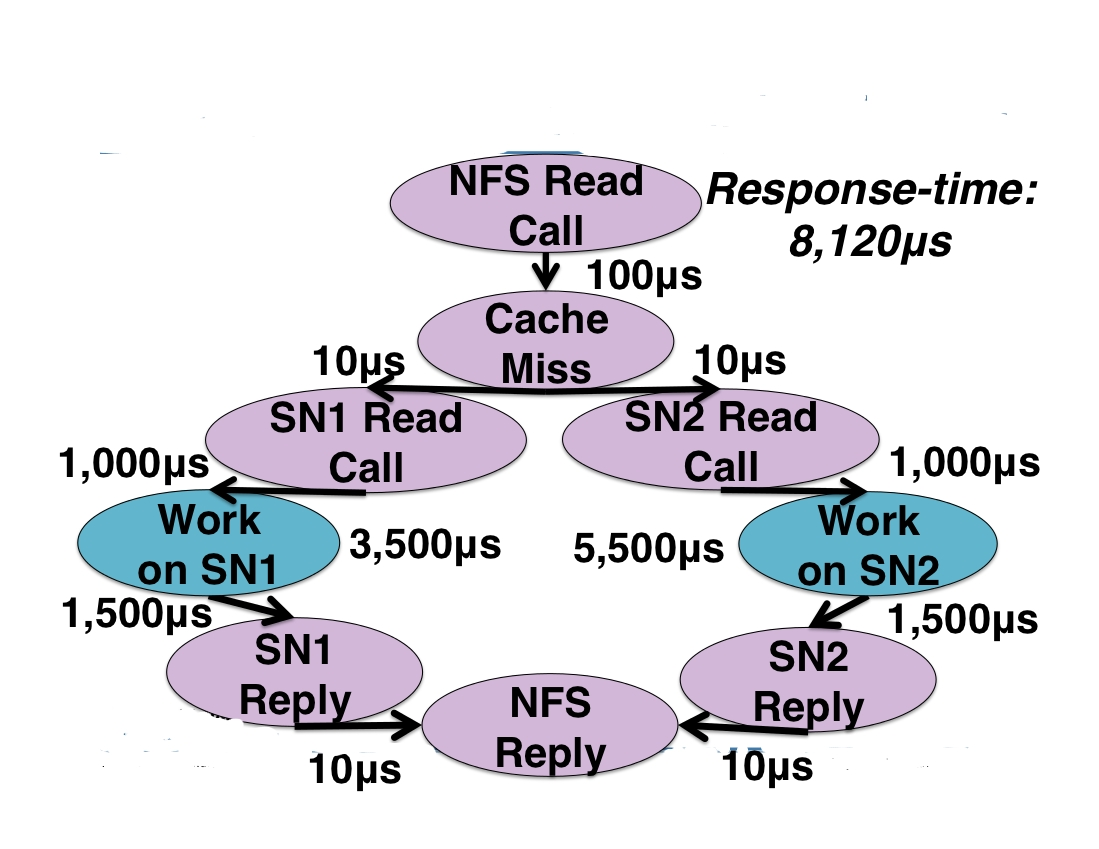
\includegraphics[width=\textwidth,height=.9\textheight]{fig/end-to-end.jpg}
\column{.3\textwidth}
\begin{itemize}
  \item Node:trace point
  \item Edge:latency
\end{itemize}
\end{columns}
\end{frame}

\section{Categorization}
\begin{frame}
\frametitle{Spectroscope workflow (\romannumeral 2)}
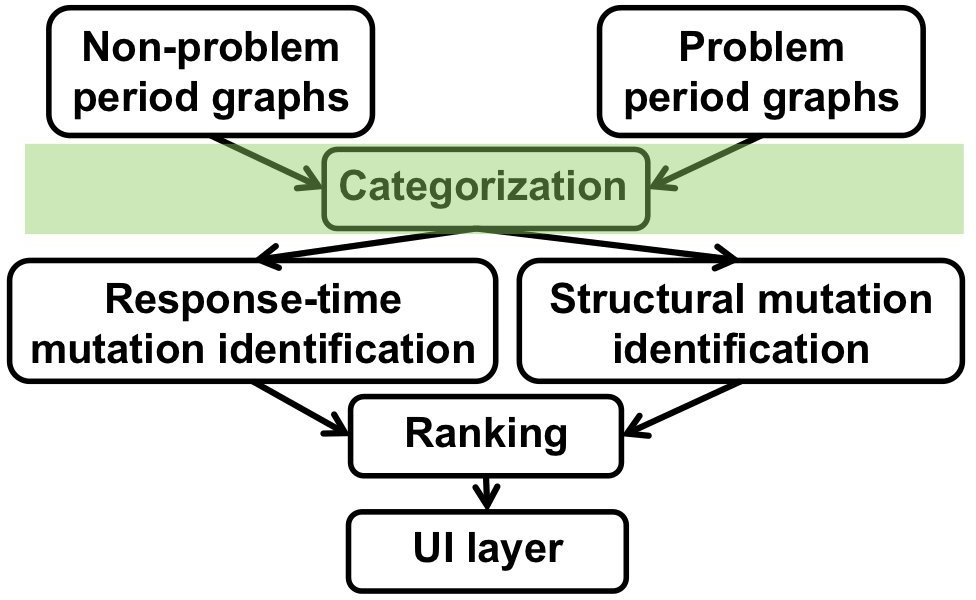
\includegraphics[width=\textwidth]{fig/work2.jpg}
\end{frame}

\begin{frame}
\frametitle{\secname}
\begin{itemize}
  \item \alert{Problem}:Even \structure{small} distributed systems can service
  hundreds to thousands of requests per second, so comparing all of
  them individually is \structure{not feasible}.
  \item It is meaningless to compare individual requests flows\pause
  \item Groups together similar request flows
  \begin{enumerate}
    \item Categories: basic unit for comparisons
    \item Allows for mutation identification by comparing per-category
    distributions
  \end{enumerate}
\end{itemize}
\end{frame}

\begin{frame}
\frametitle{What to bin into a category?}
\begin{itemize}
  \item Identically structured requests
  \begin{itemize}
    \item Uses same path/similar cost expectation
  \end{itemize}
  \vskip11pt
  \item Same path/similar costs notion is valid
  \begin{itemize}
    \item For $88-99\%$ of Ursa Minor categories
    \item For $47-69\%$ of Bigtable categories
    \begin{enumerate}
      \item Lower value due to sparser trace points
      \item Lower value also due to contention
    \end{enumerate}
  \end{itemize}
\end{itemize}
\end{frame}

\section{Identification \& Ranking}
\begin{frame}
\frametitle{Spectroscope workflow (\romannumeral 3)}
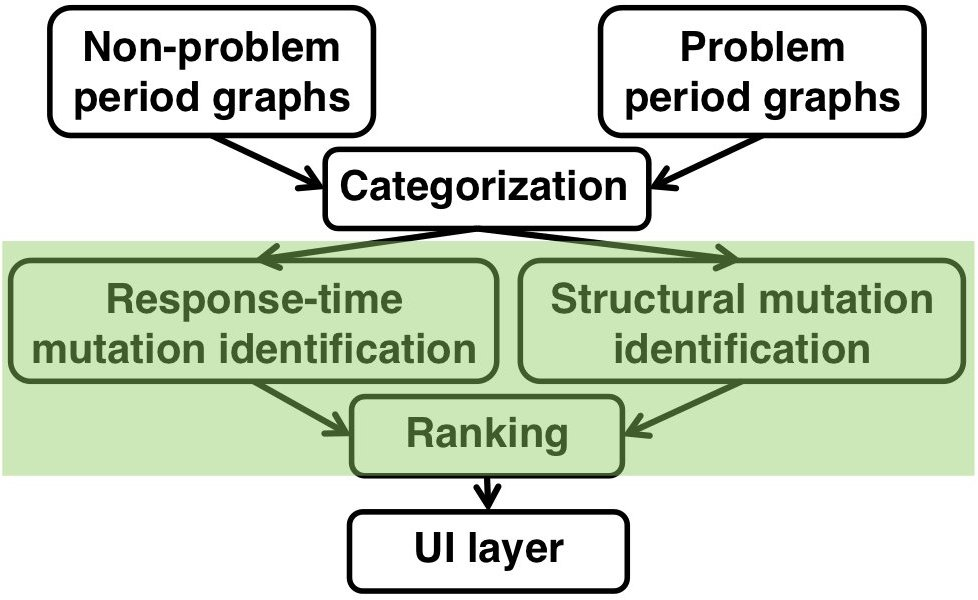
\includegraphics[width=\textwidth]{fig/work3.jpg}
\end{frame}


\begin{frame}
\frametitle{Types of Mutations}
\begin{columns}
\column{.5\textwidth}
\begin{figure}[htbp]
\centering
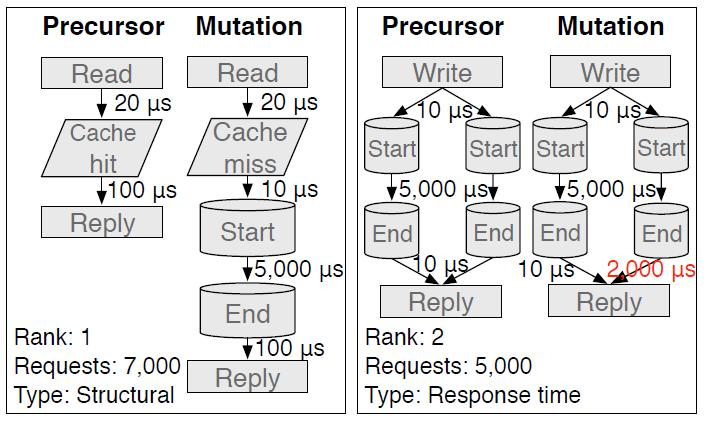
\includegraphics[width=.95\textwidth]{fig/mutation.jpg}
\caption{Types of Mutations}
\label{fig:mutation}
\end{figure}
\column{.5\textwidth}
\begin{itemize}
  \item response-time mutations
  \begin{itemize}
    \item[\ding{43}]increased cost between the periods
    \item[\ding{43}]same structure,different response time
    \vskip5pt
    \item[---] Root cause localized by
    identifying interactions responsible
  \end{itemize}
  \vskip10pt
  \item structural mutations
  \begin{itemize}
    \item[\ding{43}] different paths through the system in the problem period
    \vskip5pt
    \item[---]Root cause localized by:
    \begin{enumerate}
      \item identifying their precursors
      \item identifying how mutation \& precursor differ
    \end{enumerate}
  \end{itemize}
\end{itemize}
\end{columns}
\end{frame}

\begin{frame}
\frametitle{Identifying response-time mutations}
\shadowbox{use of Kolmogorov-Smirnov two-sample, non-parametric hypothesis
test}
\begin{itemize}
  \item Sets apart natural variance from mutations
  \item Also used to find interactions responsible
\end{itemize}
\begin{center}
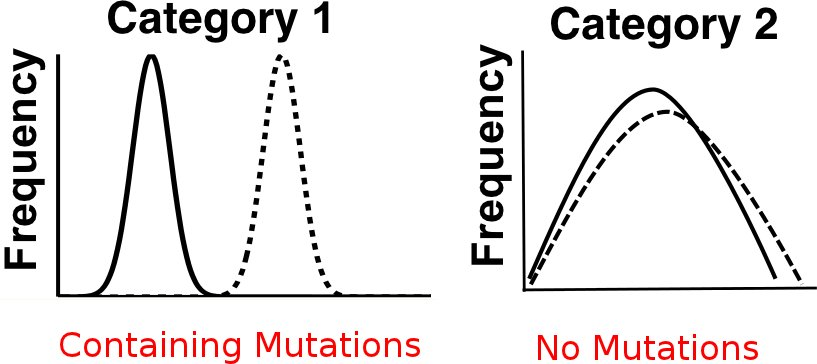
\includegraphics[width=.7\textwidth]{fig/mutation1.jpg}
\end{center}
\end{frame}

\begin{frame}
\frametitle{Identifying structural mutations}
\begin{itemize}
  \item Assume similar workloads executed
  \begin{enumerate}
    \item Categories with more problem period requests contain mutations
    \item Reverse true for precursor categories
  \end{enumerate}
  \vskip11pt
  \item \structure{Threshold} used to differentiate natural
  variance from categories mutations
\end{itemize}
\end{frame}

\begin{frame}
\frametitle{Mapping mutations to precursors}
\begin{columns}
\column{.5\textwidth}
\begin{itemize}
  \item eliminate different root nodes in precursor categories
  \item remove precursor categories having decreased in request count less than the increase in
  request count of the structure-mutation category
  \item rank remaining precursor categories according to likelihood of
  having donated requests
%   \tiny{
%   \begin{enumerate}
%     \item may be more than one problem
%     \item One problem may yield many mutations
%     \item Rank based on number of requests affected in response time
%   \end{enumerate}}
\end{itemize}
\column{.5\textwidth}
\begin{figure}[htbp]
\centering
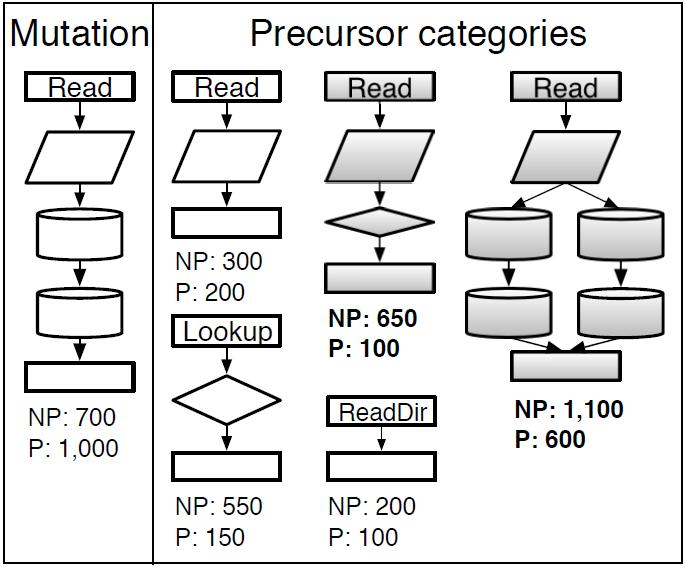
\includegraphics[width=\textwidth]{fig/mapping.jpg}
\caption{Only two categories are reserved}
\end{figure}
\end{columns}
\end{frame}

\section{Visulation}
\begin{frame}
\frametitle{Spectroscope workflow (\romannumeral 4)}
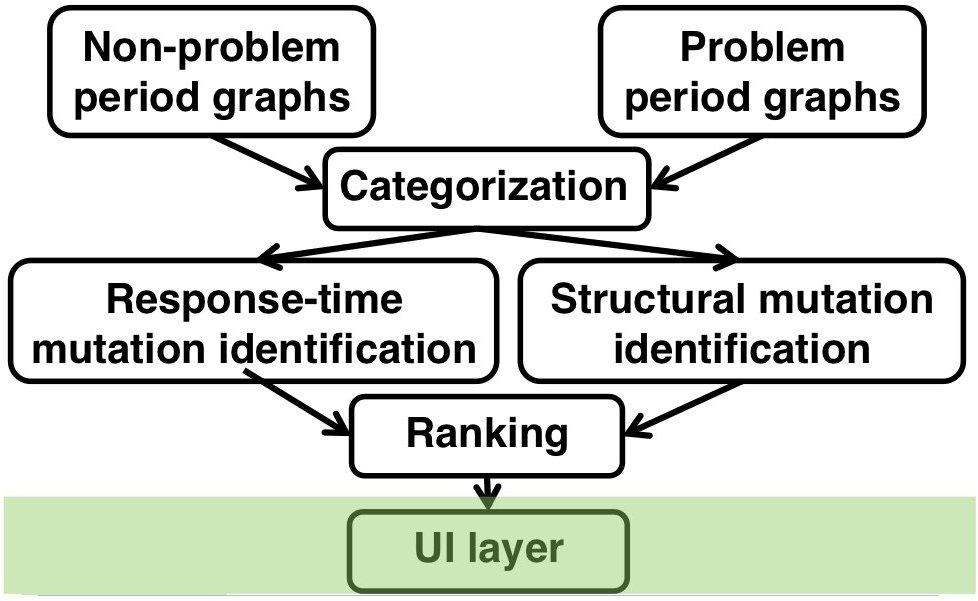
\includegraphics[width=\textwidth]{fig/work4.jpg}
\end{frame}

\begin{frame}
\frametitle{UI layer}
\only<1>{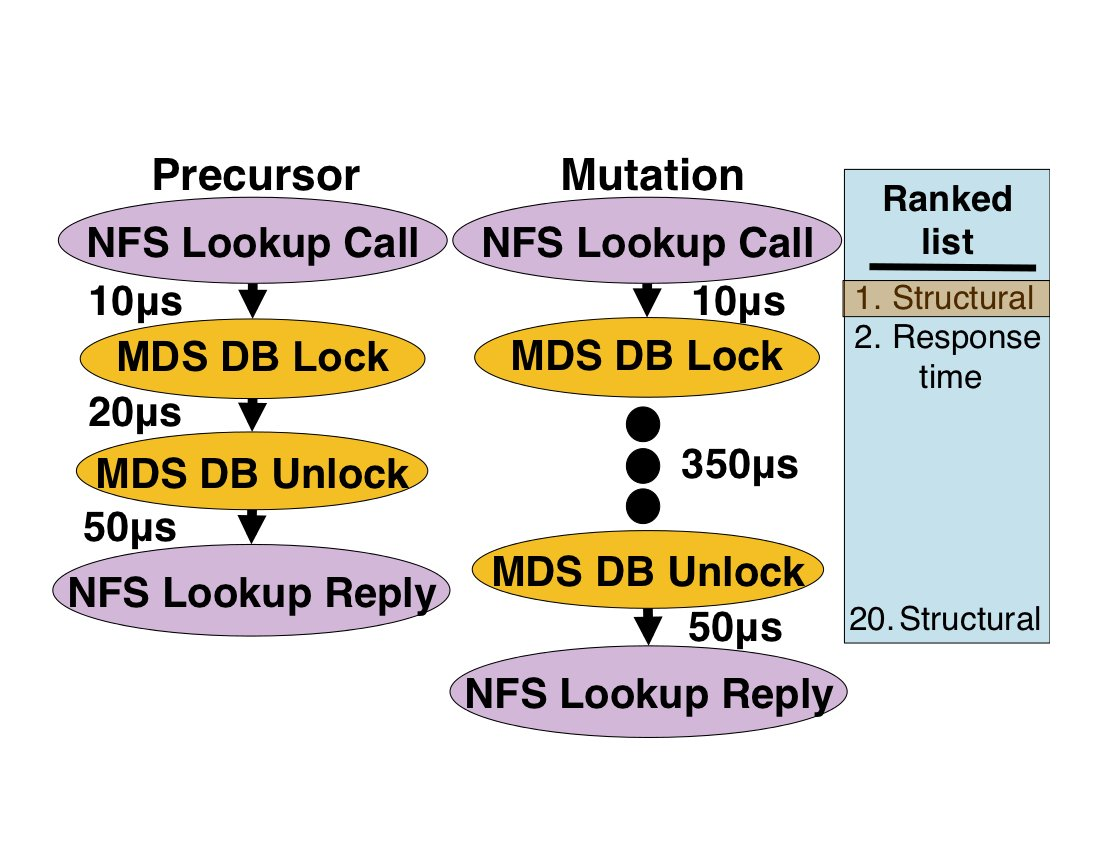
\includegraphics[width=.9\textwidth]{fig/UI0.jpg}}
\only<2>{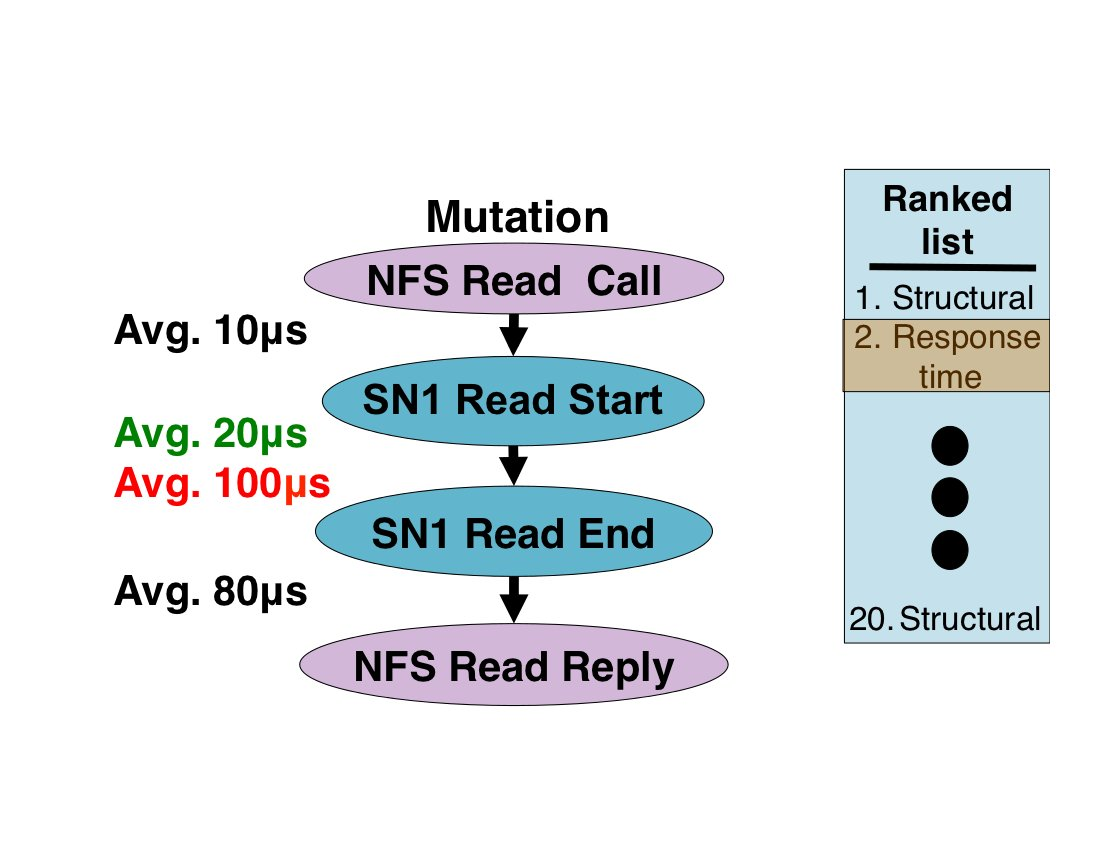
\includegraphics[width=.9\textwidth]{fig/UI1.jpg}}
\end{frame}

\part{Experiemental appratus}
\frame{\partpage}

\section{Ursa Minor case studies}
\begin{frame}
\frametitle{Methodoly}
\shadowbox{Three complementary metrics provided for evaluation}
\begin{itemize}
  \item The percentage of the 10 highest-ranked categories
  that are relevant$\left(Top\ 10 rel. \right)$
  \item The percentage of false-positive categories$\left(FPs\right)$
  \item Request coverage$\left(Cov.\right)$
\end{itemize}
\end{frame}

\begin{frame}[t]
\frametitle{Overview of the Ursa Minor case studies}
\vskip18pt
\begin{table}
\centering\tiny
\begin{tabular}{|r|r|r|r||r|r|r|}
\hline
\textbf{Name}& \textbf{Manifestation}& \textbf{Root cause}& \textbf{$\#$ of
results}& \textsl{\textbf{Top 10 rel. $\%$}}& \textsl{\textbf{FPs $\%$}}&
\textsl{\textbf{Cov.$\%$}}\\\hline
\uncover<2->{MDS config} & \uncover<2->{Structural} &
\uncover<2->{Config.
change} & \uncover<2->{128} & \uncover<2->{100} & \uncover<2->{2} &
\uncover<2->{2}\\
\uncover<3->{RMWs} & \uncover<3->{Structural} & \uncover<3->{Env. change} &
\uncover<3->{3} & \uncover<3->{100} & \uncover<3->{0} & \uncover<3->{100}\\
\uncover<4->{MDS} \uncover<4->{prefetch. $50$} & \uncover<4->{Structural} &
\uncover<4->{Internal change} & \uncover<4->{7} & \uncover<4->{29} &
\uncover<4->{71} & \uncover<4->{93}\\
\uncover<4->{MDS prefetch. $10$} & \uncover<4->{Structural} &
\uncover<4->{Internal change} & \uncover<4->{16} & \uncover<4->{70} &
\uncover<4->{56} & \uncover<4->{96}\\
\uncover<5->{Create behaviour} & \uncover<5->{Structural} & \uncover<5->{Design
problem} & \uncover<5->{11} & \uncover<5->{40} & \uncover<5->{64} &
\uncover<5->{N\slash A}\\
\uncover<6->{$100\mu s$ delay} & \uncover<6->{Response time} &
\uncover<6->{Internal change} & \uncover<6->{17} & \uncover<6->{0} &
\uncover<6->{100} & \uncover<6->{0}\\
\uncover<6->{$500\mu s$ delay} & \uncover<6->{Response time} &
\uncover<6->{Internal change} & \uncover<6->{166} & \uncover<6->{100} &
\uncover<6->{6} & \uncover<6->{92}\\
\uncover<6->{$1ms$} \uncover<6->{delay} & \uncover<6->{Response time} &
\uncover<6->{Internal change} & \uncover<6->{178} & \uncover<6->{100} &
\uncover<6->{7} & \uncover<6->{93}\\
\uncover<7->{Periodic spikes} & \uncover<7->{No change} & \uncover<7->{Env.
change} & \uncover<7->{N\slash A} & \uncover<7->{N\slash A} &
\uncover<7->{N\slash A} & \uncover<7->{N\slash A}\\
\hline
\end{tabular}
\end{table}
\vskip15pt
\only<2>
{
\ovalbox{MDS{~\footnote{Metadata Server}} configuration change}\vskip5pt
\begin{itemize}
  \item used Spectroscope to compare request flows between two runs of
  \textit{postmark-large}, one from before the check-in and one from after.
\end{itemize}
}
\only<3>
{
\ovalbox{Read-modify-writes}\vskip5pt
Compare request flows between a run of \textit{IoZone}
in which
\begin{itemize}
  \item the Linux client's I\slash O size was set to 16KB and
  \item the Linux client's I\slash O size was set to 4KB
\end{itemize}
}
\only<4>
{\hypertarget{evaluation}
\ovalbox{MDS prefetching}\beamergotobutton{\hyperlink{prefetching}{Jump to
Graph}}\vskip5pt
\begin{itemize}
  \item Compared two runs of \textit{linux-build}, one with prefetching disabled
  and another with it enabled.
  \item \textsf{SM\_THRESHOLD} set to be $50$,$10$ respectively.
\end{itemize}
}
\only<5>
{
\ovalbox{Create behaviour}\vskip5pt
\begin{itemize}
  \item To serve a CREATE, the metadata server executed
  a tight inter-component loop with a storage node
  \item Categories containing \emph{structural mutations} executed this loop more
  times than their precursor categories
\end{itemize}
}
\only<6>
{
\ovalbox{Slowdown due to code changes}\vskip5pt
\begin{itemize}
  \item Compare request flows between two runs of \textit{SFS97}.
  \item Injecting $100\mu s$, $500\mu s$, and $1ms$ spin loops
\end{itemize}
}
\only<7>
{
\ovalbox{Periodic spikes}\vskip5pt
Currently suspect the problem to be backup activity initiated from
the facilities department.
}
\end{frame}

\section{Experiences at Google}
\begin{frame}
\frametitle{\secname}
\begin{itemize}
  \item Inter-cluster performance
  \item Performance change in a large service
  \vskip15pt
  \item[\ding{46}] Challenges remain in scaling request-flow
  comparison techniques to large distributed services
\end{itemize}
\end{frame}

\appendix
\begin{frame}
\frametitle{Summary}
\begin{block}{}
\begin{itemize}
  \item Introduced request-flow comparison as a new way to diagnose perform
  changes
  \vskip5pt
  \item Presented algorithms for localizing problems by identifying mutations
  \vskip5pt
  \item Showed utility of our approach by using it to diagnose real, unsolved
  problems
\end{itemize}
\end{block}
\end{frame}

\newcount\opaqueness
\begin{frame}
\itshape
\animate<1-5>
\Large

\only<1-5>{
\animatevalue<1-5>{\opaqueness}{20}{100}
\begin{colormixin}{\the\opaqueness!averagebackgroundcolor}
\begin{centering}
\Huge\color{red} Thank You for your attention!\par
\end{centering}
\end{colormixin}
}
\end{frame}
\end{document}
